\chapter{Netzwerk-Spiel}
\label{chapter:netzwerkspiel}
% \begin{figure}[H]
%     \centering
%     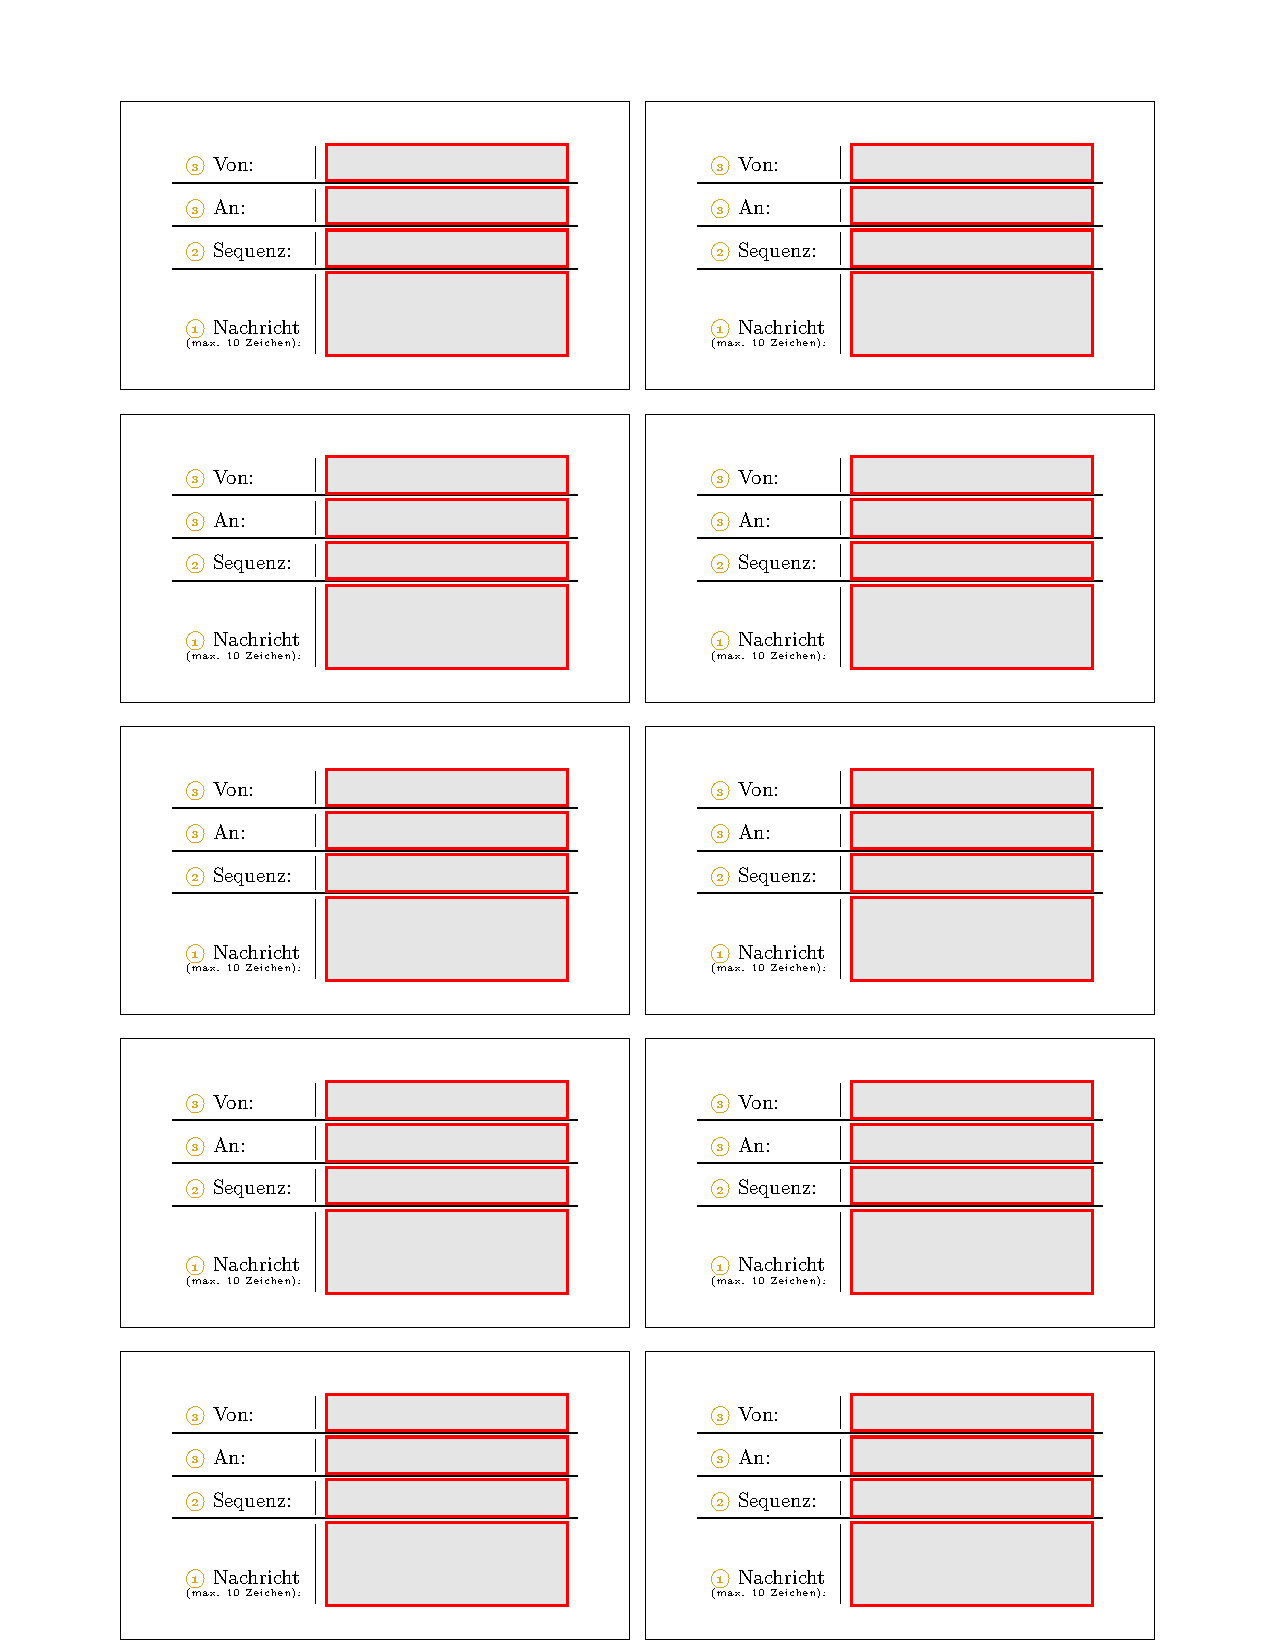
\includegraphics[width=.7\textwidth]{Grundlagen_Info/07_Netzwerke/Skript/Appendices/Zettel.pdf}
%     \caption{Zettel für das Netzwerk-Spiel}
% \end{figure}
% \clearpage

In dieser Übung sollen Sie die verschiedenen Schichten des Netzwerk-Schichtenmodells anhand eines praktischen Beispiels anwenden. Dabei schicken Sie sich gegenseitig Nachrichten zu, indem sie die \gls{IP}-Adresse der anderen Person verwenden. Die \gls{IP}-Adresse wurde im Vorfeld von der Lehrperson zugeteilt, welche ebenfalls die Rolle des Routers (innerhalb eines lokalen Netzwerks) übernimmt. Das Spiel läuft wie folgt ab:

\begin{enumerate}
	\item Jede Person erhält ein ausgedrucktes Namensschild mit dazugehöriger, zufällig generierter \gls{MAC}-Adresse, sowie einer \gls{IP}-Adresse. Das Namensschild wird so platziert, dass es für alle gut sichtbar ist.
	\item Die Lehrperson erklärt die verschiedenen Schichten des Netzwerk-Schichtenmodells und wie sie in diesem Spiel angewendet werden.
	\item Jede Person schreibt eine kurze Nachricht (z.B. \enquote{Hallo, wie geht's?}) und adressiert sie an eine andere Person, indem sie deren \gls{IP}-Adresse verwendet. Die maximale Nachrichtenlänge beträgt 10 Zeichen.
	\item Die Nachricht wird mit einer Sequenznummer versehen, um die Reihenfolge der Nachrichten zu kennzeichnen (Couvert Grösse \texttt{A6}).
	\item  Die Nachricht wird nun mit der \gls{IP}-Adresse des Empfängers sowie der eigenen \gls{IP}-Adresse versehen und dem Router übergeben.
	\item Der Router kennt nur die \gls{MAC}-Adressen der Teilnehmer und muss die \gls{IP}-Adressen in \gls{MAC}-Adressen auflösen, um die Nachricht korrekt weiterzuleiten. Er tut dies, indem er alle laut fragt, wer eine bestimmte \gls{IP}-Adresse hat und konsultiert dabei seine \gls{ARP}-Tabelle. Falls eine Nachricht nicht den Regeln entspricht (z.B. zu lange Nachricht, falsche IP-Adresse), wird sie verworfen und nicht weitergeleitet. Ansonsten leitet der Router die Nachricht an den entsprechenden Empfänger weiter.
	\item Die Empfänger öffnen die Couvert-Nachrichten und sortieren die Nachrichten nach Sequenz-Nummer. Sie lesen die Nachrichten laut vor und beantworten sie gegebenenfalls.
	\item Die Lehrperson fasst die Übung zusammen und erklärt, wie das Netzwerk-Schichtenmodell in der Praxis funktioniert. Dabei wird auf die verschiedenen Schichten eingegangen und erläutert, wie sie in diesem Spiel umgesetzt wurden.
	\item Optional: Die Lehrperson kann die Übung erweitern, indem sie verschiedene Netzwerk-Szenarien simuliert, z.B. Netzwerk-Ausfälle, Verzögerungen oder Störungen, um die Auswirkungen auf die Kommunikation zu verdeutlichen.
	\item Mögliche Erweiterung des Spiels: zweiter und dritter Router (Personen) bestimmen, um die Konzepte von Subnetzen und Routing zu verdeutlichen. Konzepte: Netzmaske, Gateway, Interface, Routing-Tabelle.
\end{enumerate}
\clearpage

\thispagestyle{empty}
\newgeometry{margin=.5cm}

\newcommand{\zettel}[1]{
	\fbox{
		\begin{minipage}[t][4cm][t]{0.47\textwidth}
			\begin{table}[H]
				\centering
				\small
				\begin{tabular}{p{3cm}|l}
					\rowcolor{\networkLayerColor!20}\coin{3} Von:                                      & \texttt{\TextField[width=4cm, print, borderwidth=0, backgroundcolor=, height=.3cm]{}}   \\\midrule
					\rowcolor{\networkLayerColor!20}\coin{3} An:                                       & \texttt{\TextField[width=4cm, print,borderwidth=0, backgroundcolor=, height=.3cm]{}}   \\\midrule
					\rowcolor{\transportLayerColor!20}\coin{2} Sequenz:                                  & \texttt{\TextField[width=4cm, print,borderwidth=0, backgroundcolor=, height=.3cm]{}}   \\\midrule
					\rowcolor{\applicationLayerColor!20}\coin{1} Nachricht\newline\tiny (max. 10 Zeichen): & \TextField[width=4cm,height=.7cm, print,borderwidth=0, backgroundcolor=]{} \\
				\end{tabular}
			\end{table}
		\end{minipage}
	}
}

\begin{table}[H]
	\begin{tabular}{cc}
		\zettel & \zettel \\
		\\
		\zettel & \zettel \\
		\\
		\zettel & \zettel \\
		\\
		\zettel & \zettel \\
		\\
		\zettel & \zettel \\
		\\
		\zettel & \zettel \\
	\end{tabular}
\end{table}

\clearpage
\restoregeometry